
\newcommand{\FigBentSolenoidRelativeDrift}{
\begin{figure}[t]
\centering
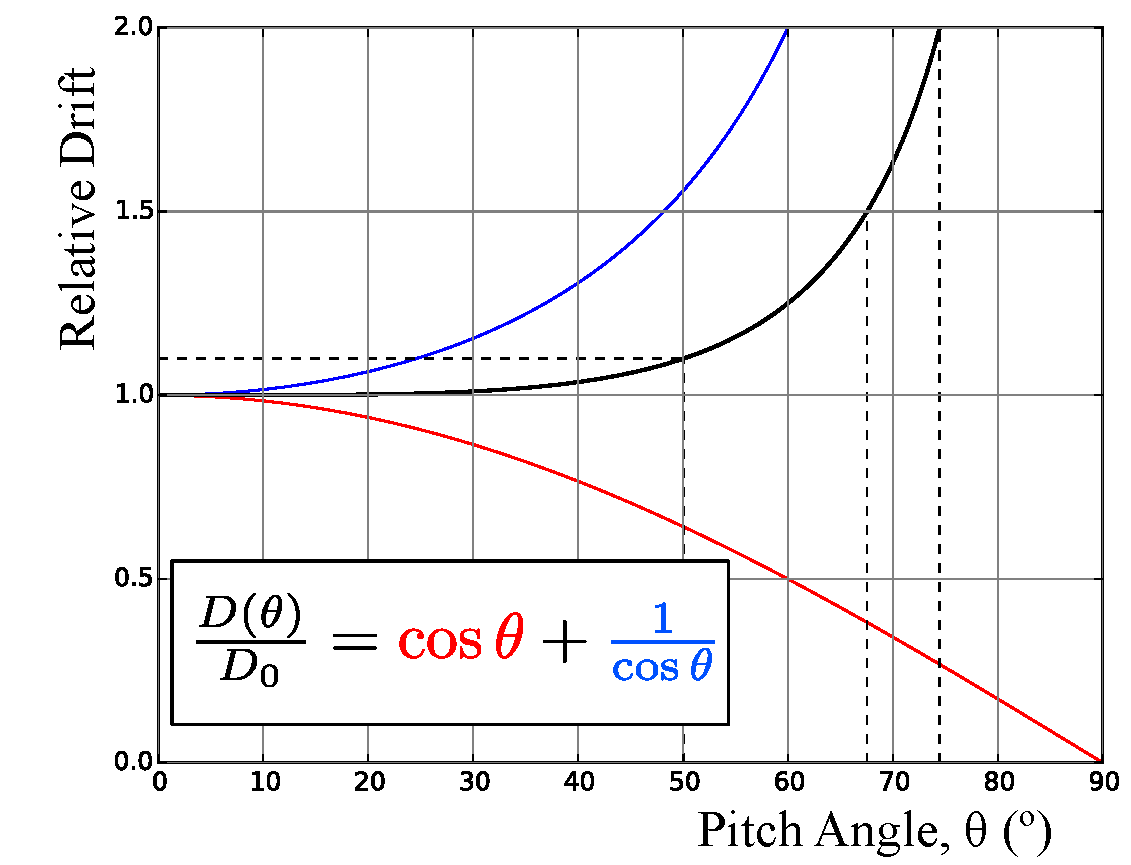
\includegraphics[width=0.6\textwidth]{figs/detector/BentSolenoids_RelativeDrift}
\caption{
Angular dependence of the magnitude of vertical drift in a bent solenoid field.
The total variation (black) remains below 10\% for pitch angles below 50\degree.
}
\figlabel{detector:bent-solenoids:angularDependence}
\end{figure}
}

\newcommand{\FigPhaseII}{
\begin{figure}[t]
\centering
%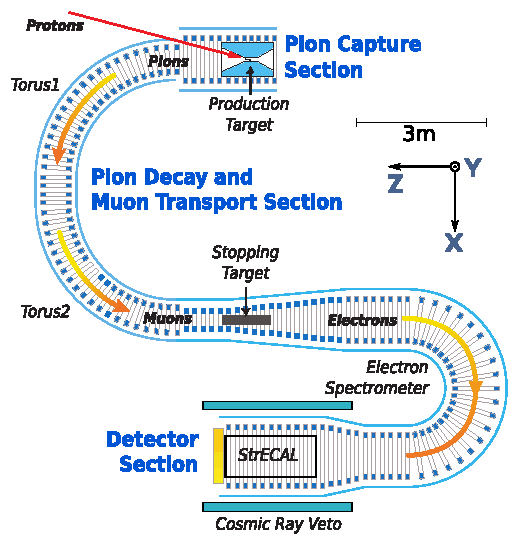
\includegraphics[width=0.9\textwidth]{figs/detector/PhaseII_schematic}
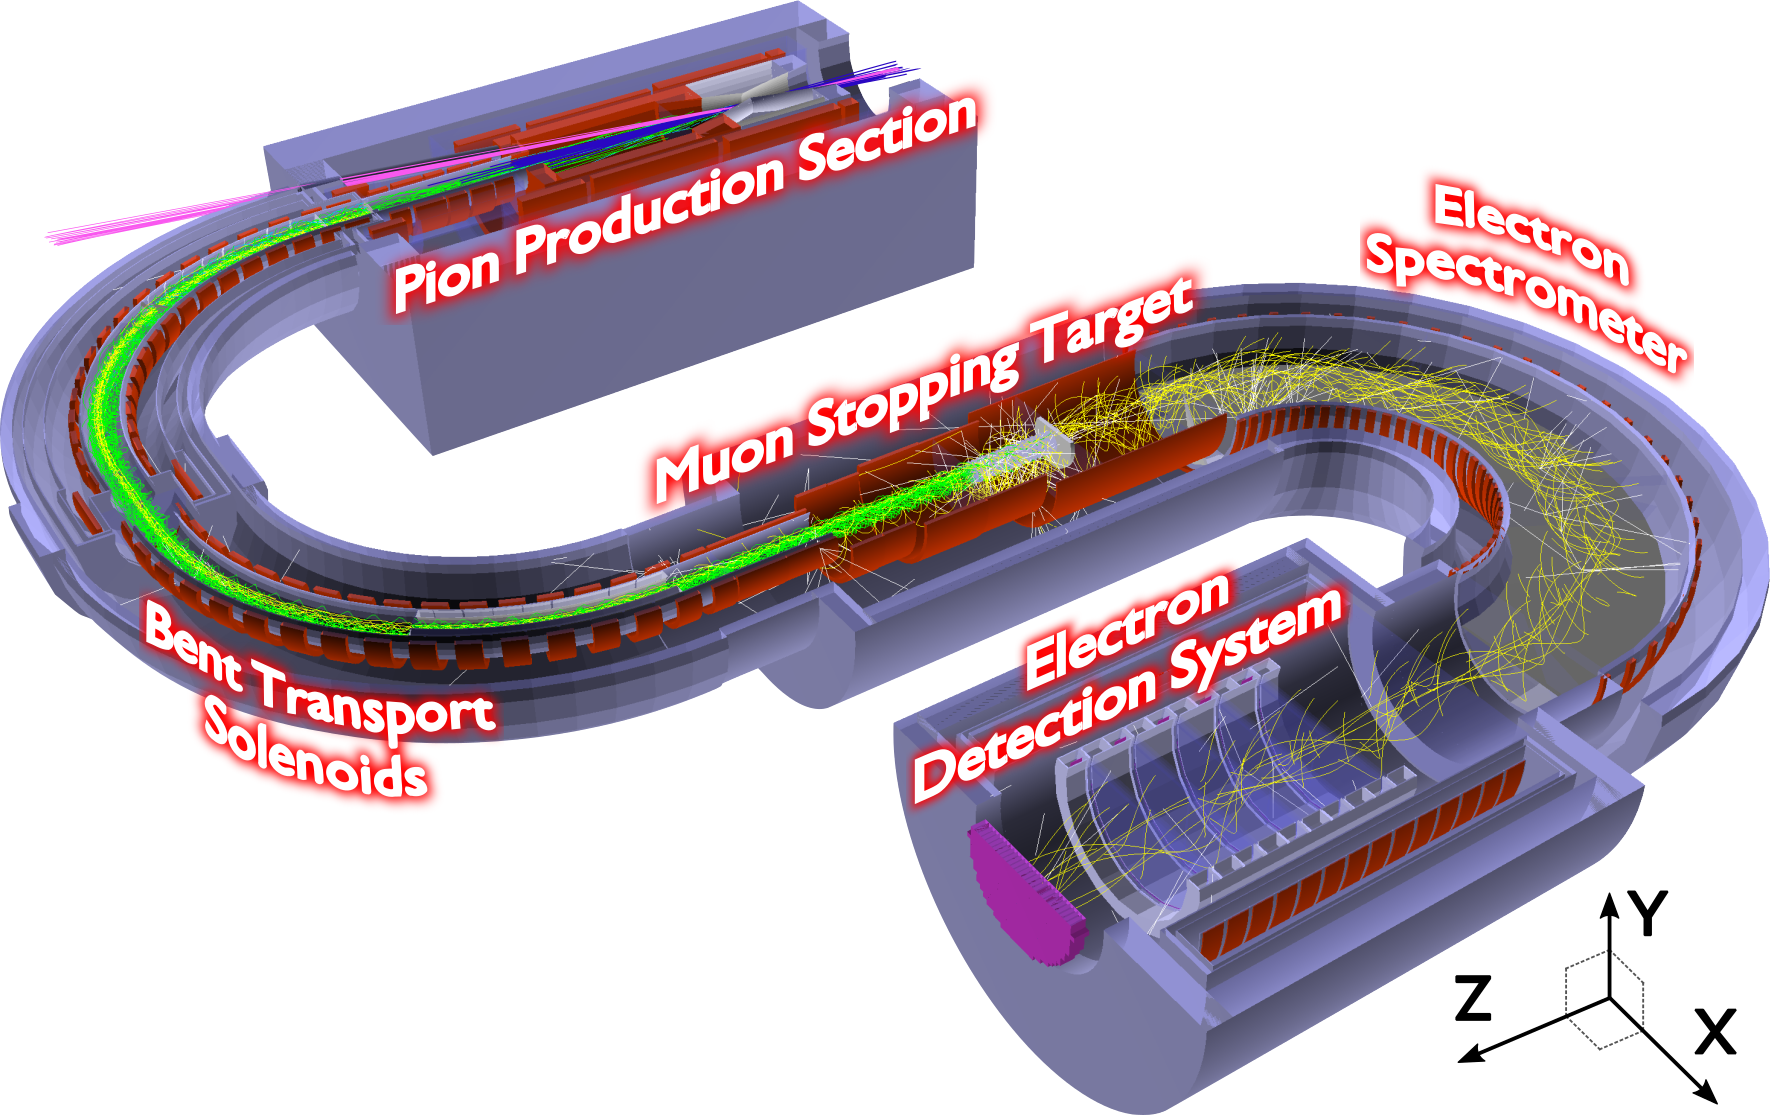
\includegraphics[width=0.9\textwidth]{figs/detector/COMET_phaseII-annotated-further}
\caption{
Schematic layout of COMET \phaseII. 
The 8 GeV proton beam (magenta) enters from the top-left, producing (amongst other things) pions (dark blue).
Pions and muons (green) travelling backwards with respect to the proton beam are then transported around 180 degrees of bent solenoid, during which time most of the pions decay producing an intense muon beam.
About 40\% of these muons then stop in the stopping target (centre of image).
Any electrons (yellow) coming from  \mueconv are then transported through another 180 degrees of bent solenoid into the detector system.
Also shown in this image is the global COMET coordinate system, with the Z-direction parallel to the beam axis at the production target and the Y-direction vertical.
}
\figlabel{detector:PhaseII:setup}
\end{figure}
}

\newcommand{\FigPhaseI}{
\begin{figure}[t]
\centering
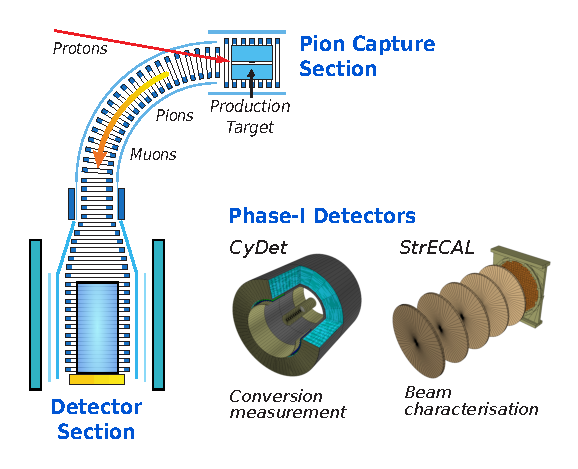
\includegraphics[height=0.4\textheight]{figs/detector/PhaseI_schematic}
\caption{
Schematic layout of COMET \phaseI including the two detector systems that will run separately, being swapped in and out of the detector solenoid depending on the study.
}
\figlabel{detector:PhaseI:setup}
\end{figure}
}

\newcommand{\TabBackgroundSummary}{
\begin{table}
\centering
%	\renewcommand{\arraystretch}{1} % Default value: 1
\begin{tabular}{lld{5}d{5}}
     \hline
     \hline\\[-1.8ex]
     Type           & Background & \multicolumn{2}{c}{Number of events during run} \\
		    &  & \multicolumn{1}{c}{\phaseI \cite{TDR2016}} & \multicolumn{1}{c}{\phaseII\cite{CDRphase2}\hspace{-0.5cm}{}~} \\
     \hline\\[-1.8ex]
     Intrinsic & Muon Decay-in-Orbit                       & 0.01              & 0.15    \\
               & Radiative Muon Capture                    & 0.0019            & <0.001  \\
               & $\mu^-$ Capture w/ n Emission             & <0.001            & <0.001  \\
               & $\mu^-$ Capture w/ Charged Part. Emission & <0.001            & <0.001  \\
     Prompt    & Radiative Pion Capture                    & 0.00028           & 0.05    \\
               & Beam Electrons                            & \multicolumn{1}{c}{\multirow{3}{*}{$\Bigg\}\le0.0038$}\hspace{4pt}{}~} & <0.1^*  \\
               & Muon Decay in Flight                      &         & <0.0002 \\
               & Pion Decay in Flight                      &                  & <0.0001 \\
               & Neutron Induced                           & \multicolumn{1}{c}{$\sim10^{-9}$\hspace{1ex}{}~}          & 0.024   \\
%               & Other beam induced B.G.                   & <2.8\times10^{-6} & -       \\
     Delayed   & Delayed Radiative Pion Capture            & \sim0             & 0.002   \\
               & Antiproton Induced                       & 0.0012            & 0.007   \\
               & Other delayed B.G.                        & \sim0             & -       \\
	Cosmic    & Cosmic Ray Muons                          & \multicolumn{1}{c}{\multirow{2}{*}{$\bigg\}\le0.01$}\hspace{17pt}{}~}                 & 0.002   \\
               & Electrons from Cosmic Ray Muons           &                   & 0.002   \\
     \hline\\[-1.8ex]
     \multicolumn{2}{c}{Total background}                  & <0.032            & <0.34    \\
     \multicolumn{2}{c}{Signal (Assuming $B=1\times10^{-16}$)} & 0.31          & 3.8     \\
     \hline
     \hline
\end{tabular}
\caption{
	Backgrounds for COMET \phaseI (from the 2016 TDR~\cite{TDR2016}) and \phaseII (from the 2009 CDR~\cite{CDRphase2}).
	Prompt backgrounds arise by protons that occur in between bunches and are therefore suppressed by the extinction factor.
	For \phaseI, the recently measured value of $10^{-12}$ was used for the extinction factor, but for \phaseII the older expectation of $10^{-9}$ was used.
        If this is not taken into account, the \phaseI estimates suggest a greater background to signal sensitivity than for \phaseII.
        $*$) Result was statistically limited.
}
\tablabel{detector:backgrounds}%
\end{table}%
}

\newcommand{\FigPionSpectraVsAngle}{
\begin{figure}[t]
\centering
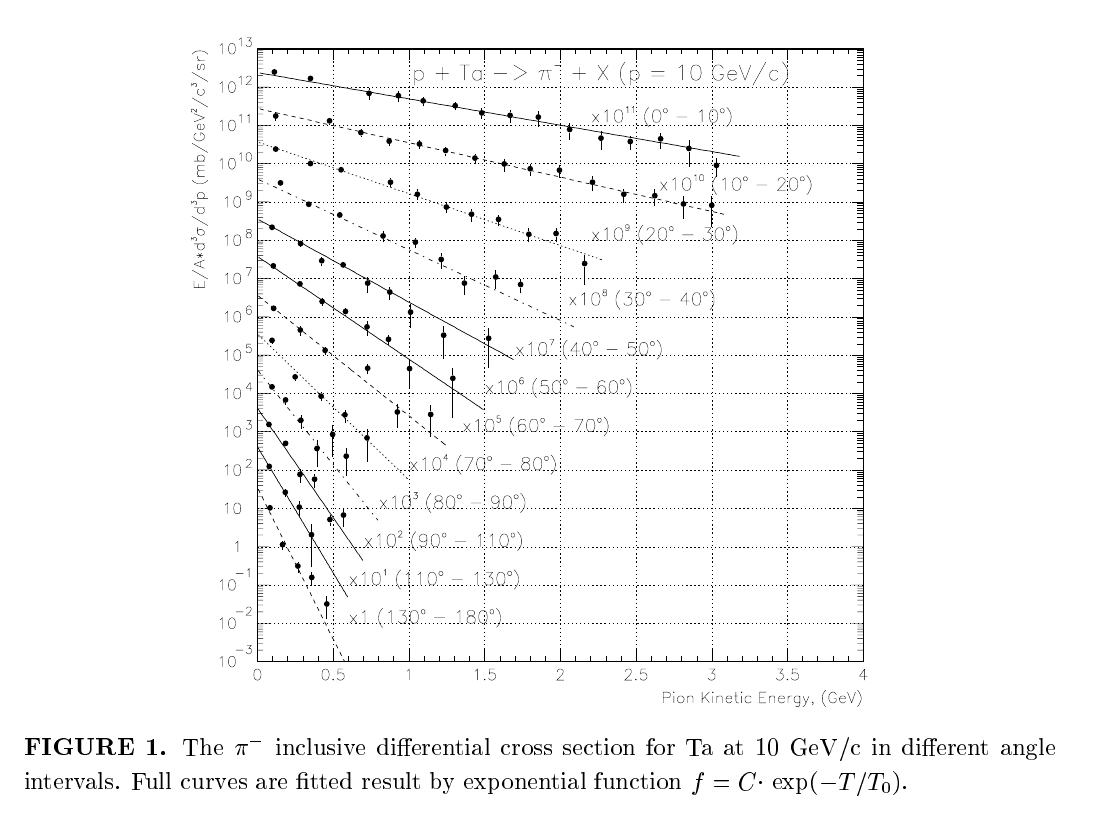
\includegraphics[width=0.8\textwidth,trim=5cm 2.5cm 5cm 1cm,clip=true]{figs/detector/Meco023-Fig1}
\caption{
Double differential cross section of pion production on a tantalum target from protons with 10~GeV kinetic energy~(reproduced from Meco note 23~\cite{Meco023} which itself used~\cite{Armutliiski:17710}).
It is clear that the high-energy component of the spectrum is suppressed as you move to higher production angles which is important for reducing background rates.
Note that each line is scaled an order of magnitude compared to the line below.
}
\figlabel{detector:piYield}
\end{figure}
}

\newcommand{\FigMuonNuclearParams}{
\begin{figure}[bp]
\centering
\subfloat[][\figlabel{detector:mu-nucl-params:lifetimes}Lifetimes]{
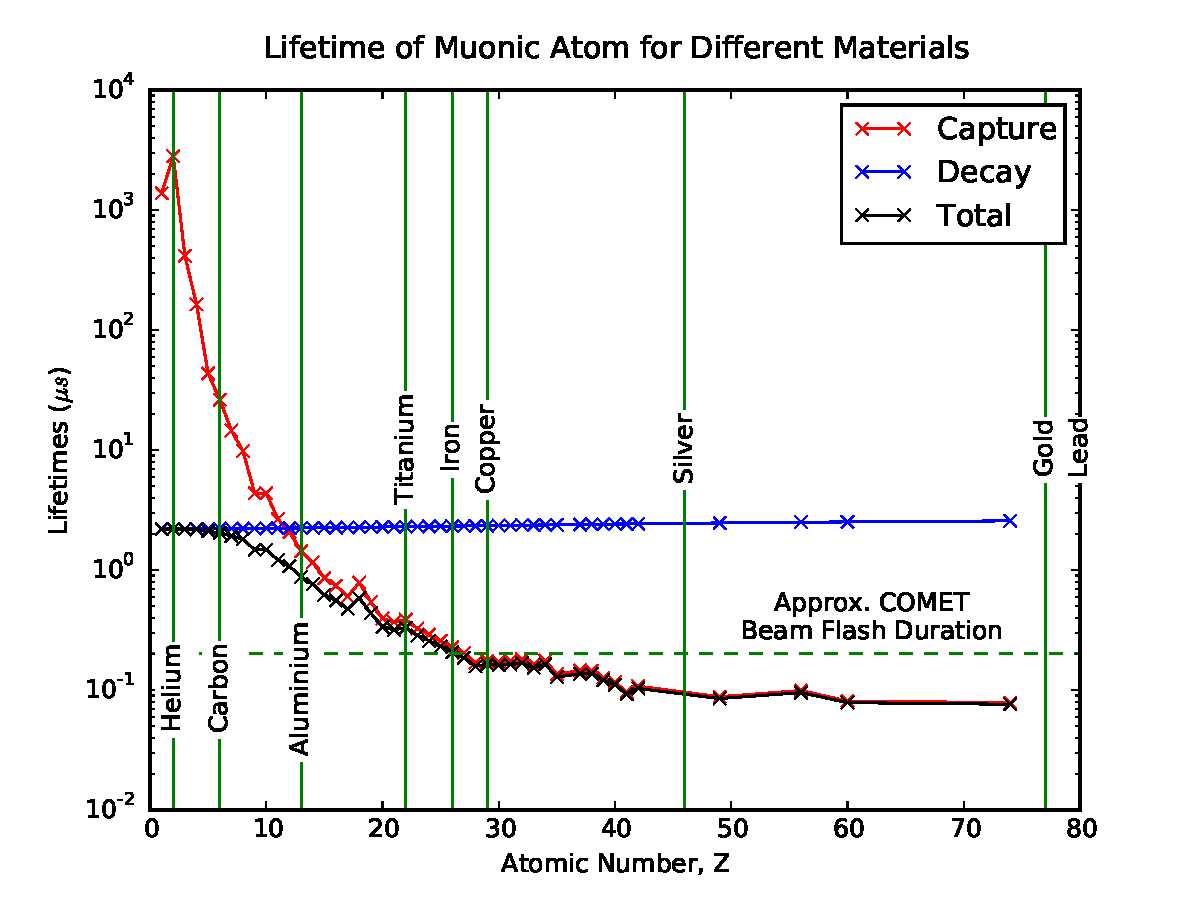
\includegraphics[width=0.85\textwidth,trim=0 0.3cm 0 0,clip]{figs/detector/MuNuclearParams_All_lifetimes.pdf}}\\
\subfloat[][\figlabel{detector:mu-nucl-params:end-point}End-point Shift]{
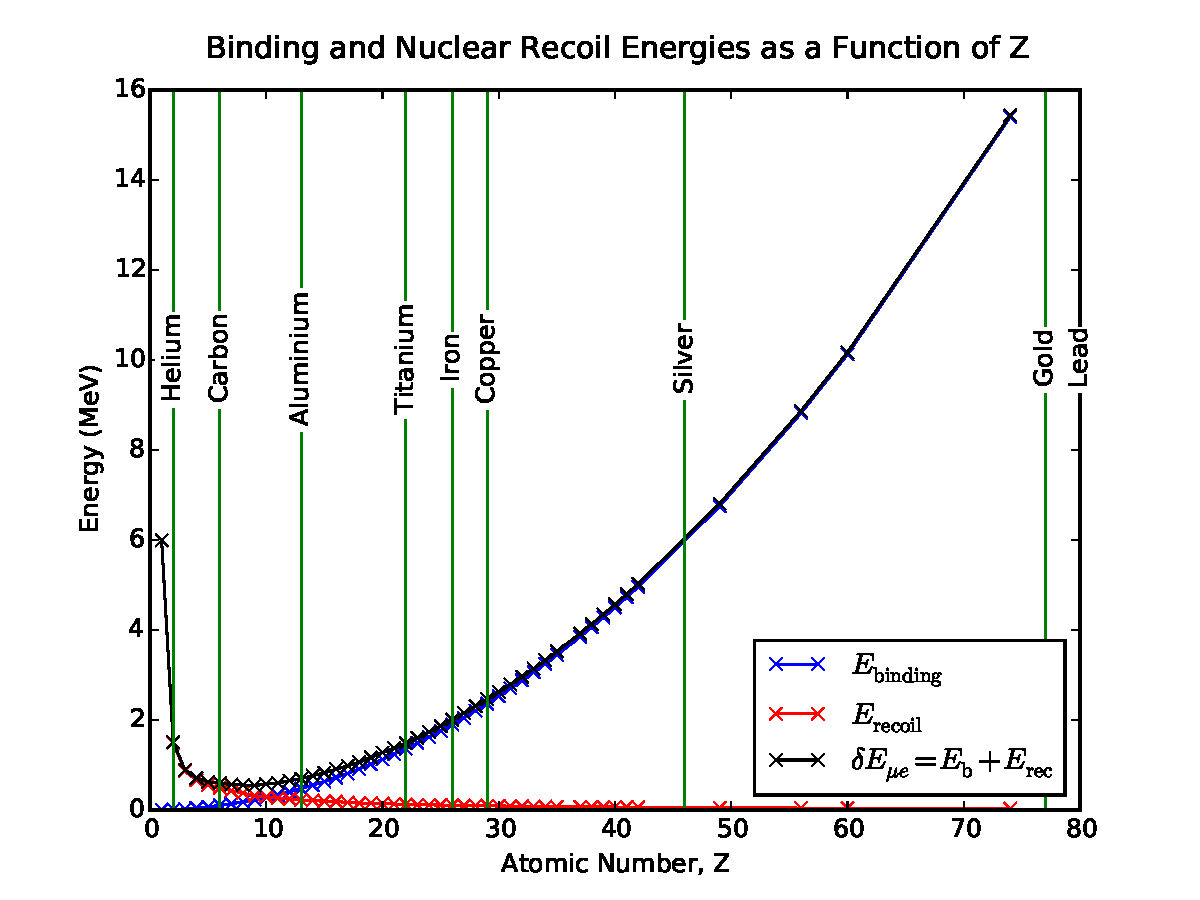
\includegraphics[width=0.42\textwidth,trim=0.1cm 0.1cm 0.9cm 1.5cm,clip]{figs/detector/MuNuclearParams_energies.pdf}}\hspace{0.02\textwidth}%
\subfloat[][\figlabel{detector:mu-nucl-params:branching-ratio}Branching Fraction]{
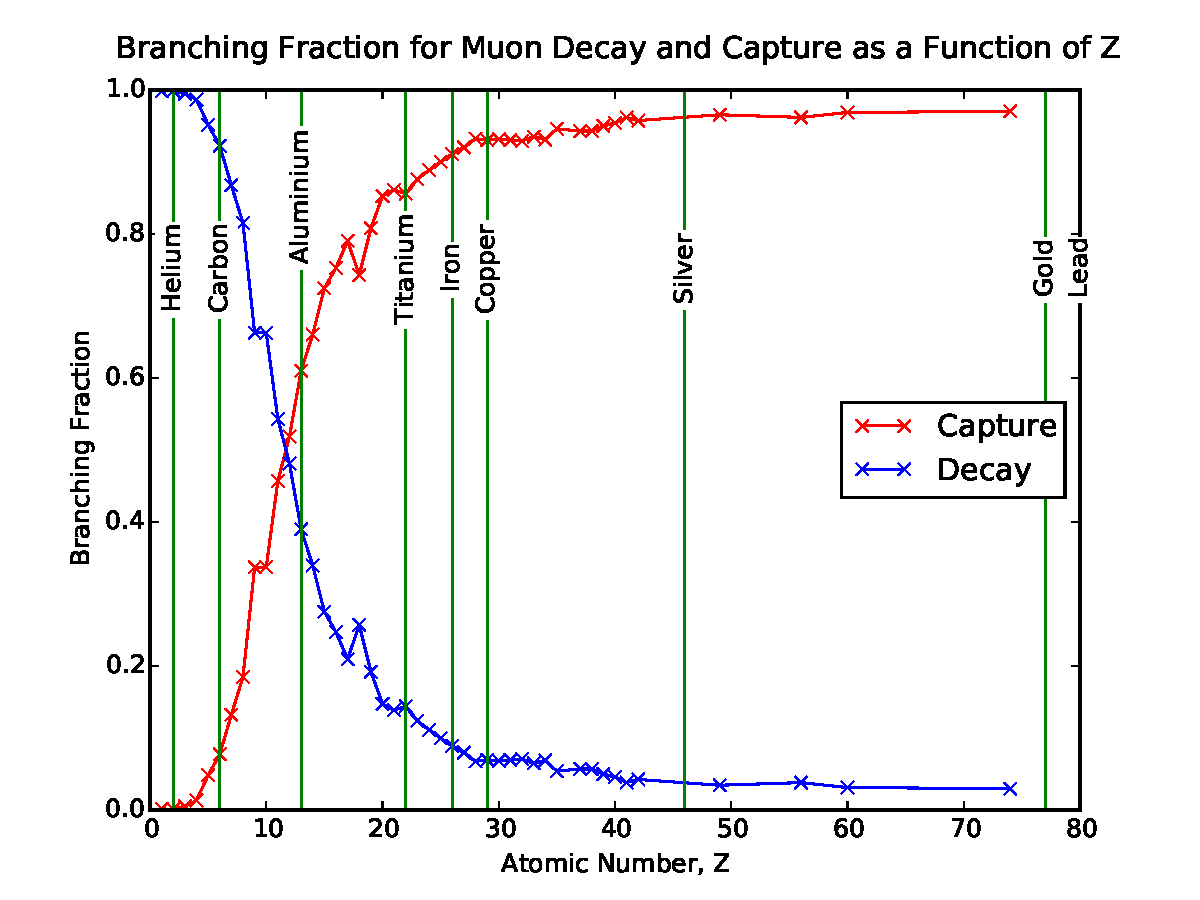
\includegraphics[width=0.42\textwidth,trim=0.1cm 0.1cm 0.9cm 1.5cm,clip]{figs/detector/MuNuclearParams_branching_fraction.pdf}}
\caption{\figlabel{detector:mu-nucl-params}
The effect of changing the atomic number on the  lifetime~\protect\subref{fig:detector:mu-nucl-params:lifetimes},
 conversion energy ( shown as $M_\mu-E_e$)~\protect\subref{fig:detector:mu-nucl-params:end-point},
 and branching ratio~\protect\subref{fig:detector:mu-nucl-params:branching-ratio}.
For the branching ratio and lifetime plots, the partial rate for muon nuclear capture and decay-in-orbit are shown separately.
The capture and decay rates are taken from the Geant4 \cite{Geant42003} parametrisation for stopped negative muons.  
Only elements for which at least 1 isotope uses a measured value are plotted.
The values for the end-point energy level are calculated using the Bohr model for the muon ground-state binding energy.
}
\end{figure}
}

\newcommand{\FigSchedule}{
\begin{figure}[b]
\centering
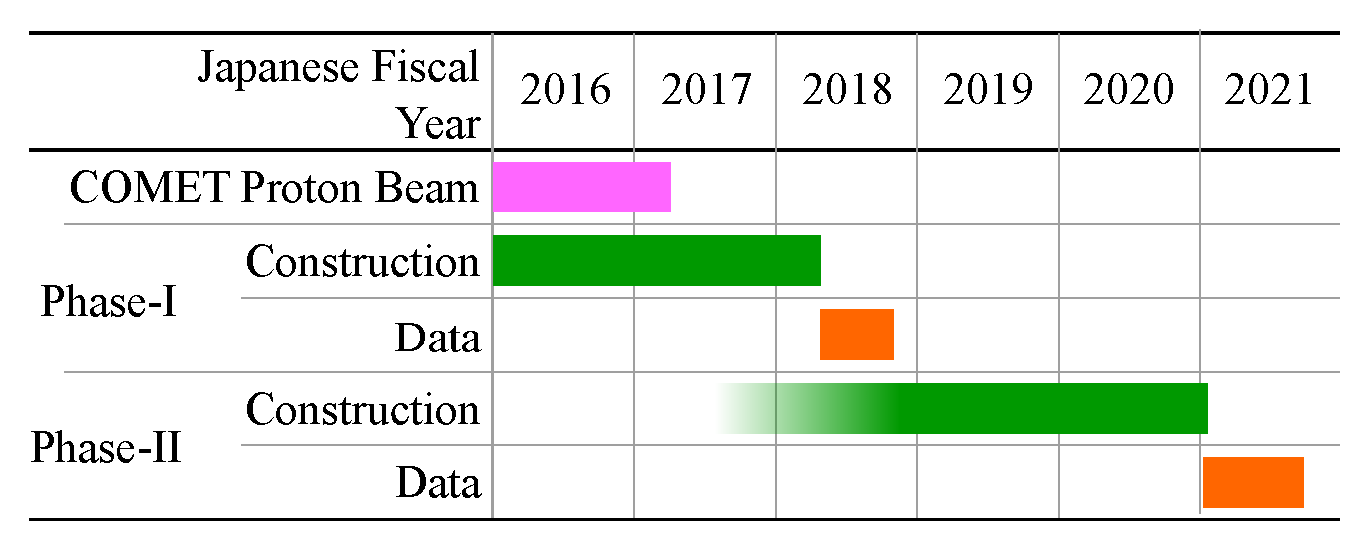
\includegraphics[width=0.95\textwidth]{figs/detector/Schedule}
\caption{
	A summarised timeline for the COMET experiment including \phaseI and \phaseII based on the 2016 TDR \cite{TDR2016}.
At the time of writing, construction of the detector solenoid is underway as well as the final stages of the facility.
}
\figlabel{detector:schedule}
\end{figure}
}

\newcommand{\FigTimingSchematic}{
\begin{figure}[b]
\centering
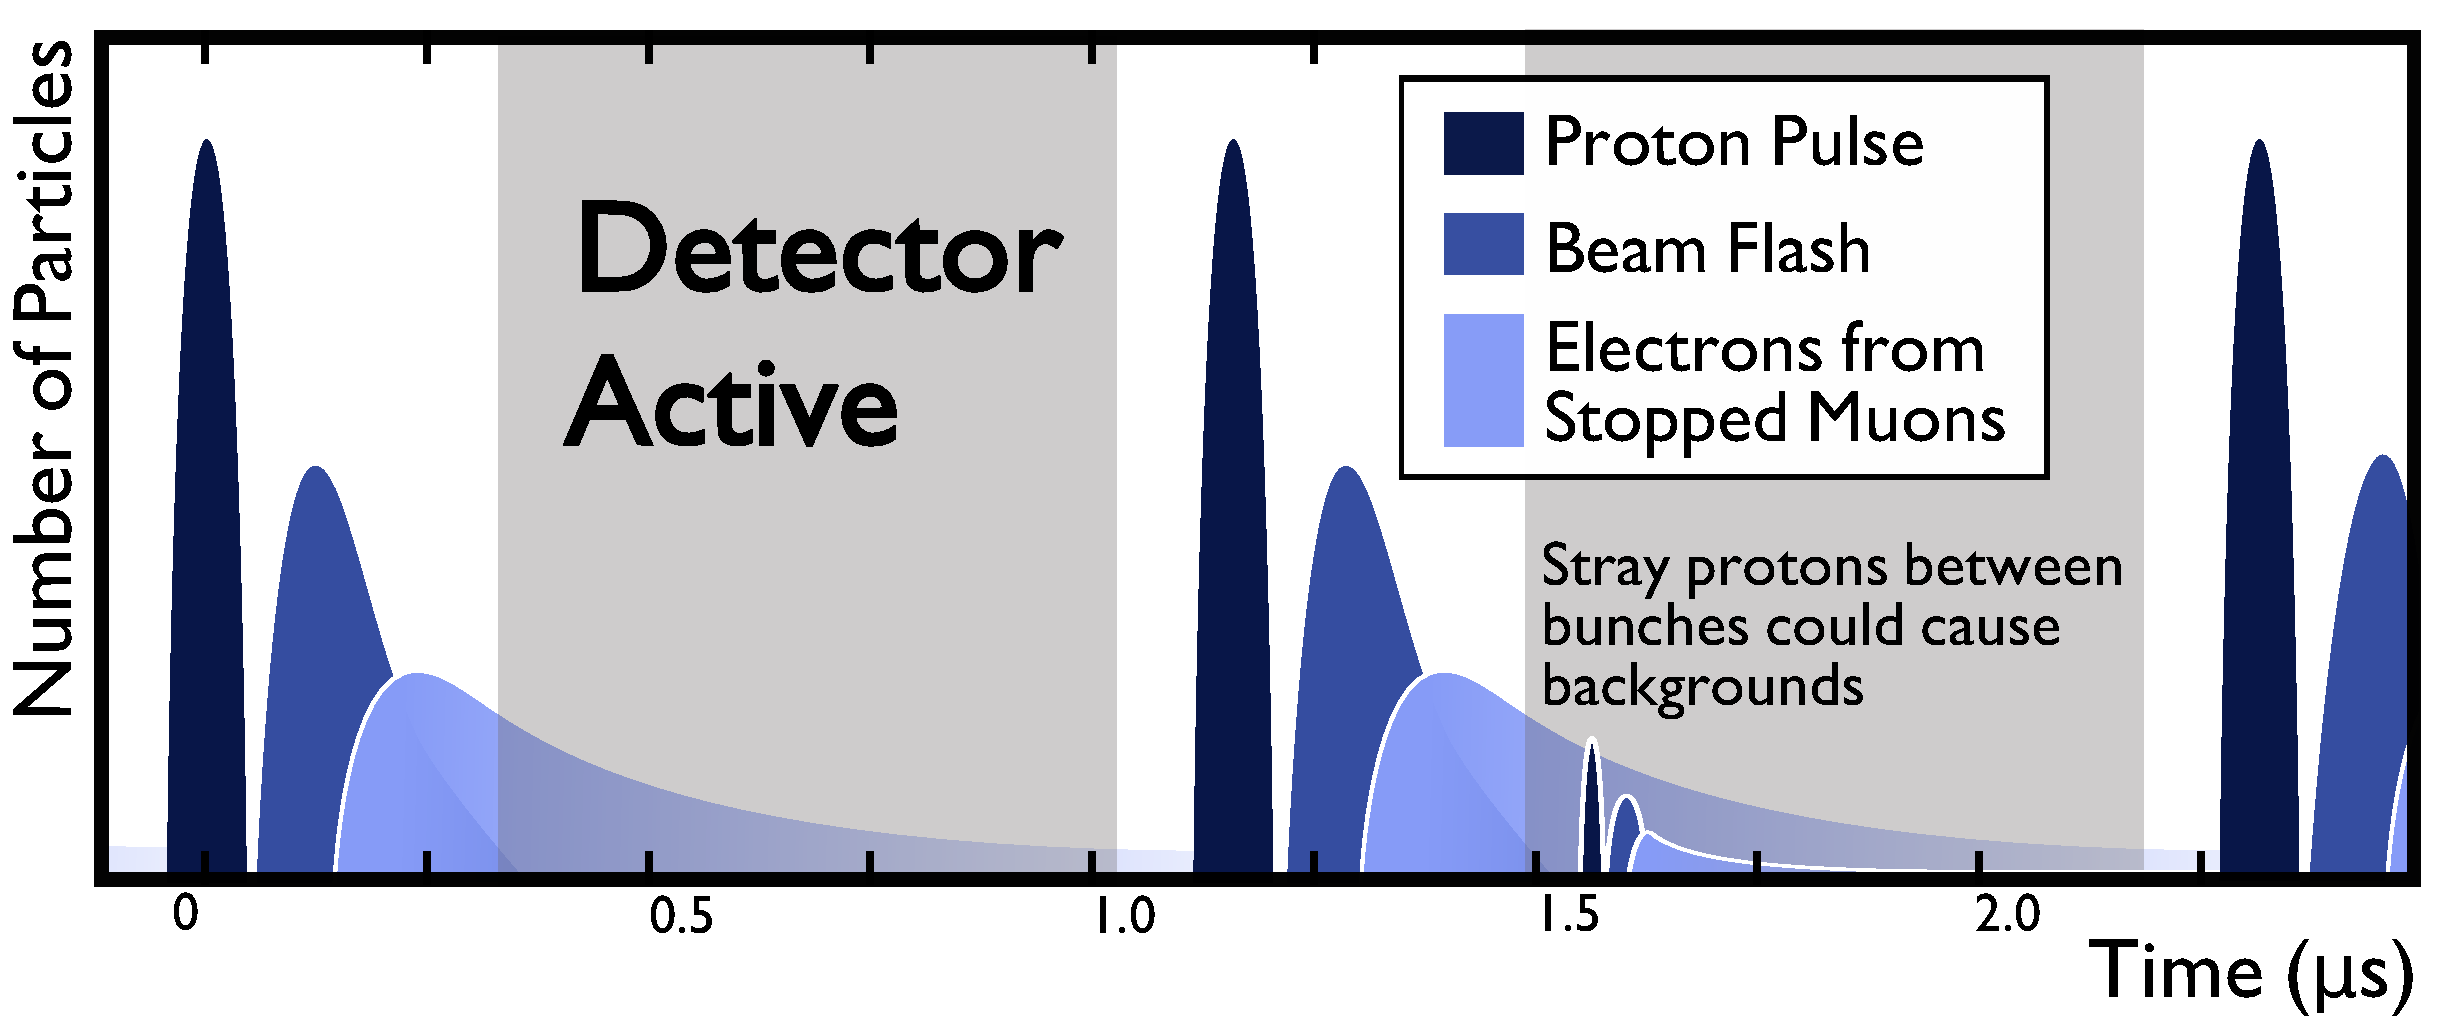
\includegraphics[width=0.95\textwidth]{figs/detector/TimingSchematic}
\caption{
Schematic for the timing structure used in the COMET experiment.
Protons arrive at the production target in 100~ns bunches separated by about 1.17~$\mu s$.
These pulses create a flash of particles in the detector which lasts for about 300~ns.
Muons that stop in the aluminium target have a lifetime of 864~ns, such that signal electrons should be detected with this timing and be well removed from the beam flash.
In between bunches there should be very few protons, or else the resultant secondaries could be detected as backgrounds.
}
\figlabel{detector:timing-schema}
\end{figure}
}


\newcommand{\FigStatusFacility}{
\begin{figure}[t]
\centering
\subfloat[][\figlabel{detector:setup:facility:foundations}Oct. 2014]{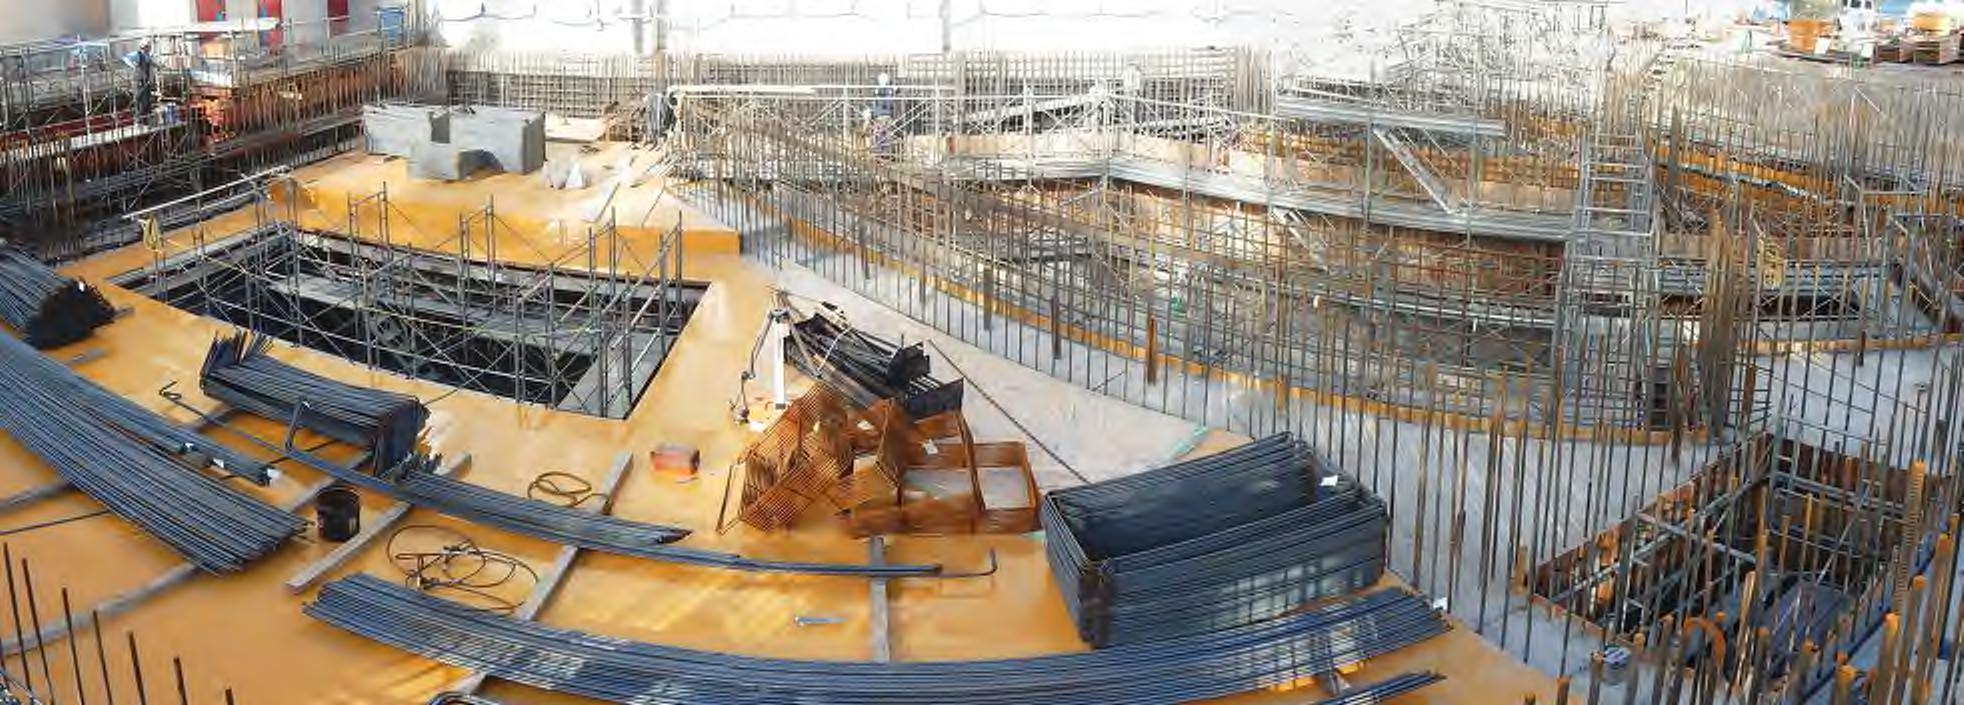
\includegraphics[width=0.8\textwidth]{figs/detector/status_photos/Hall_foundations}}\\
\subfloat[][\figlabel{detector:setup:facility:beamline}Mar. 2015]{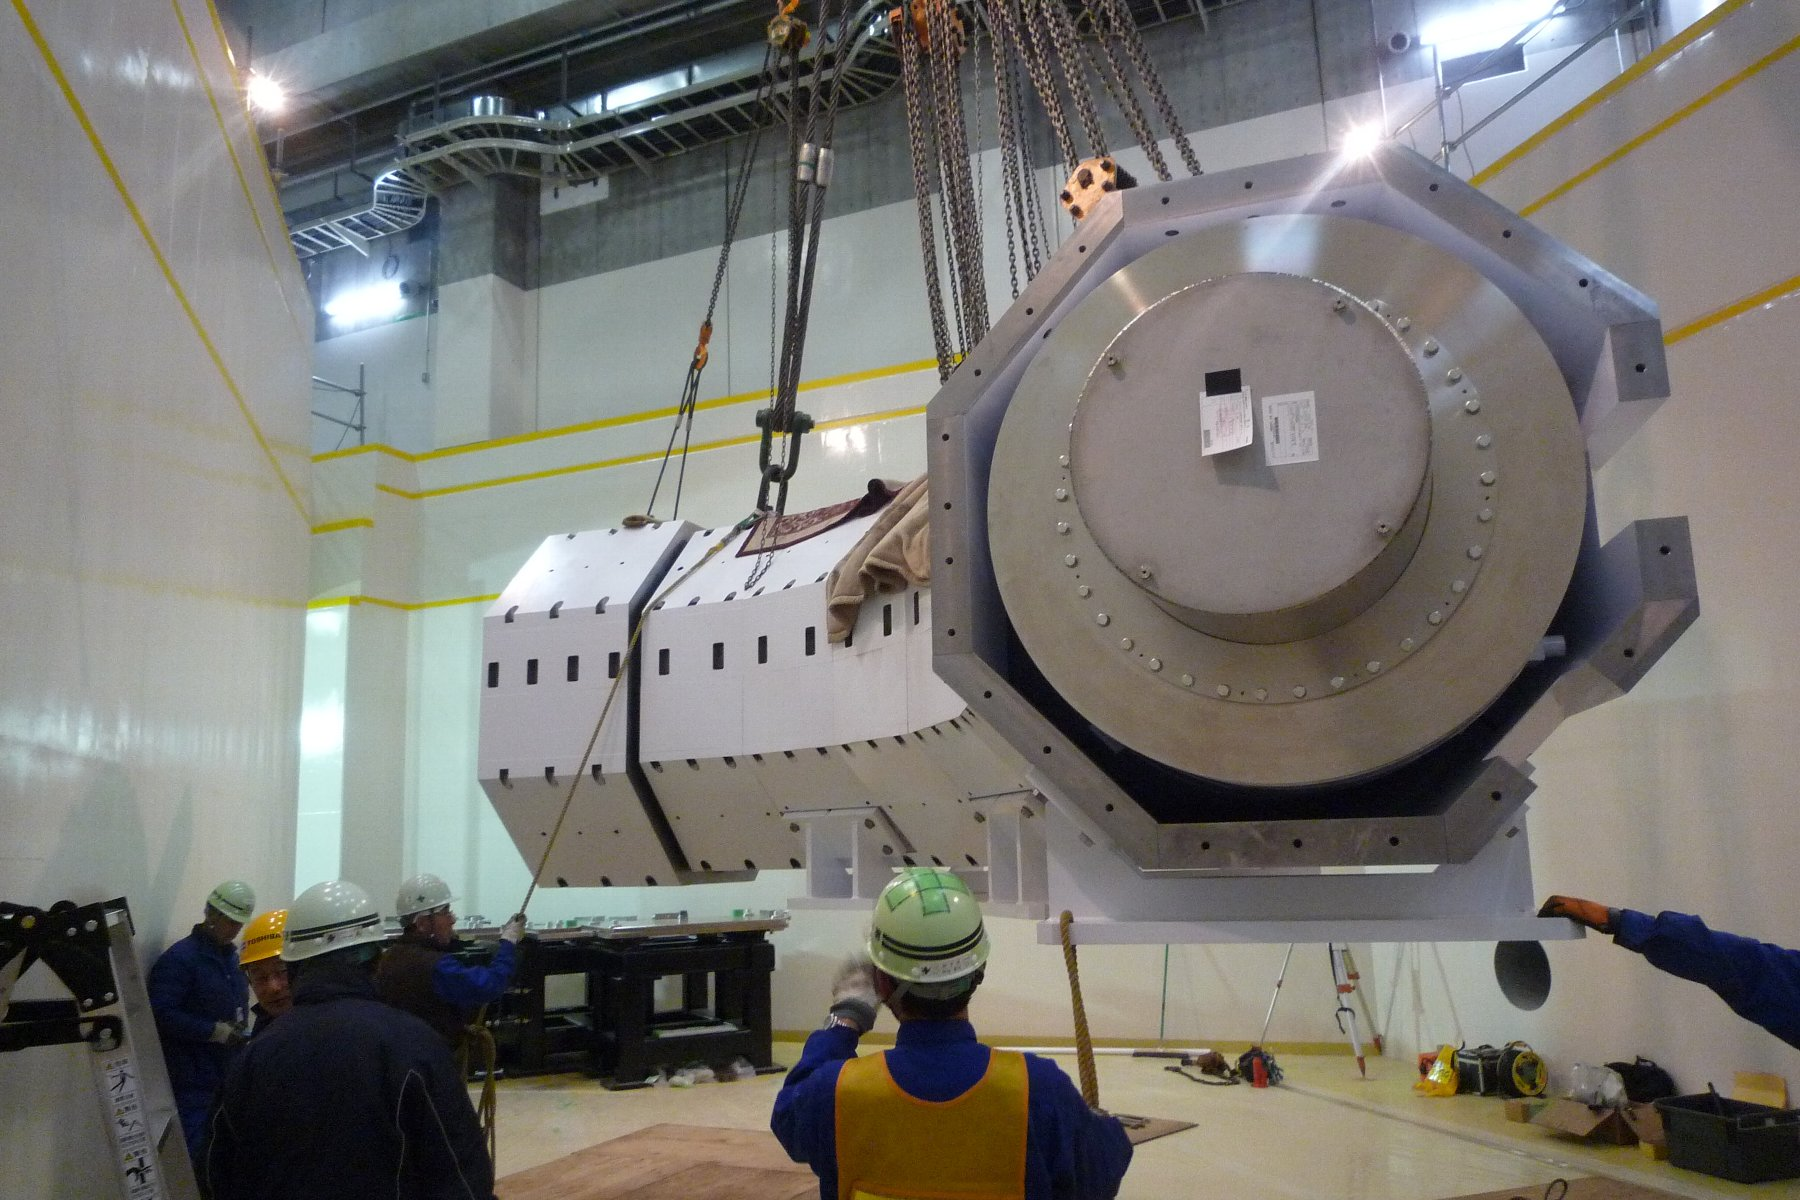
\includegraphics[width=0.52\textwidth]{figs/detector/status_photos/Hall_muBeamline}}\hspace{0.3cm}
\subfloat[][\figlabel{detector:setup:facility:me}Dec. 2015]{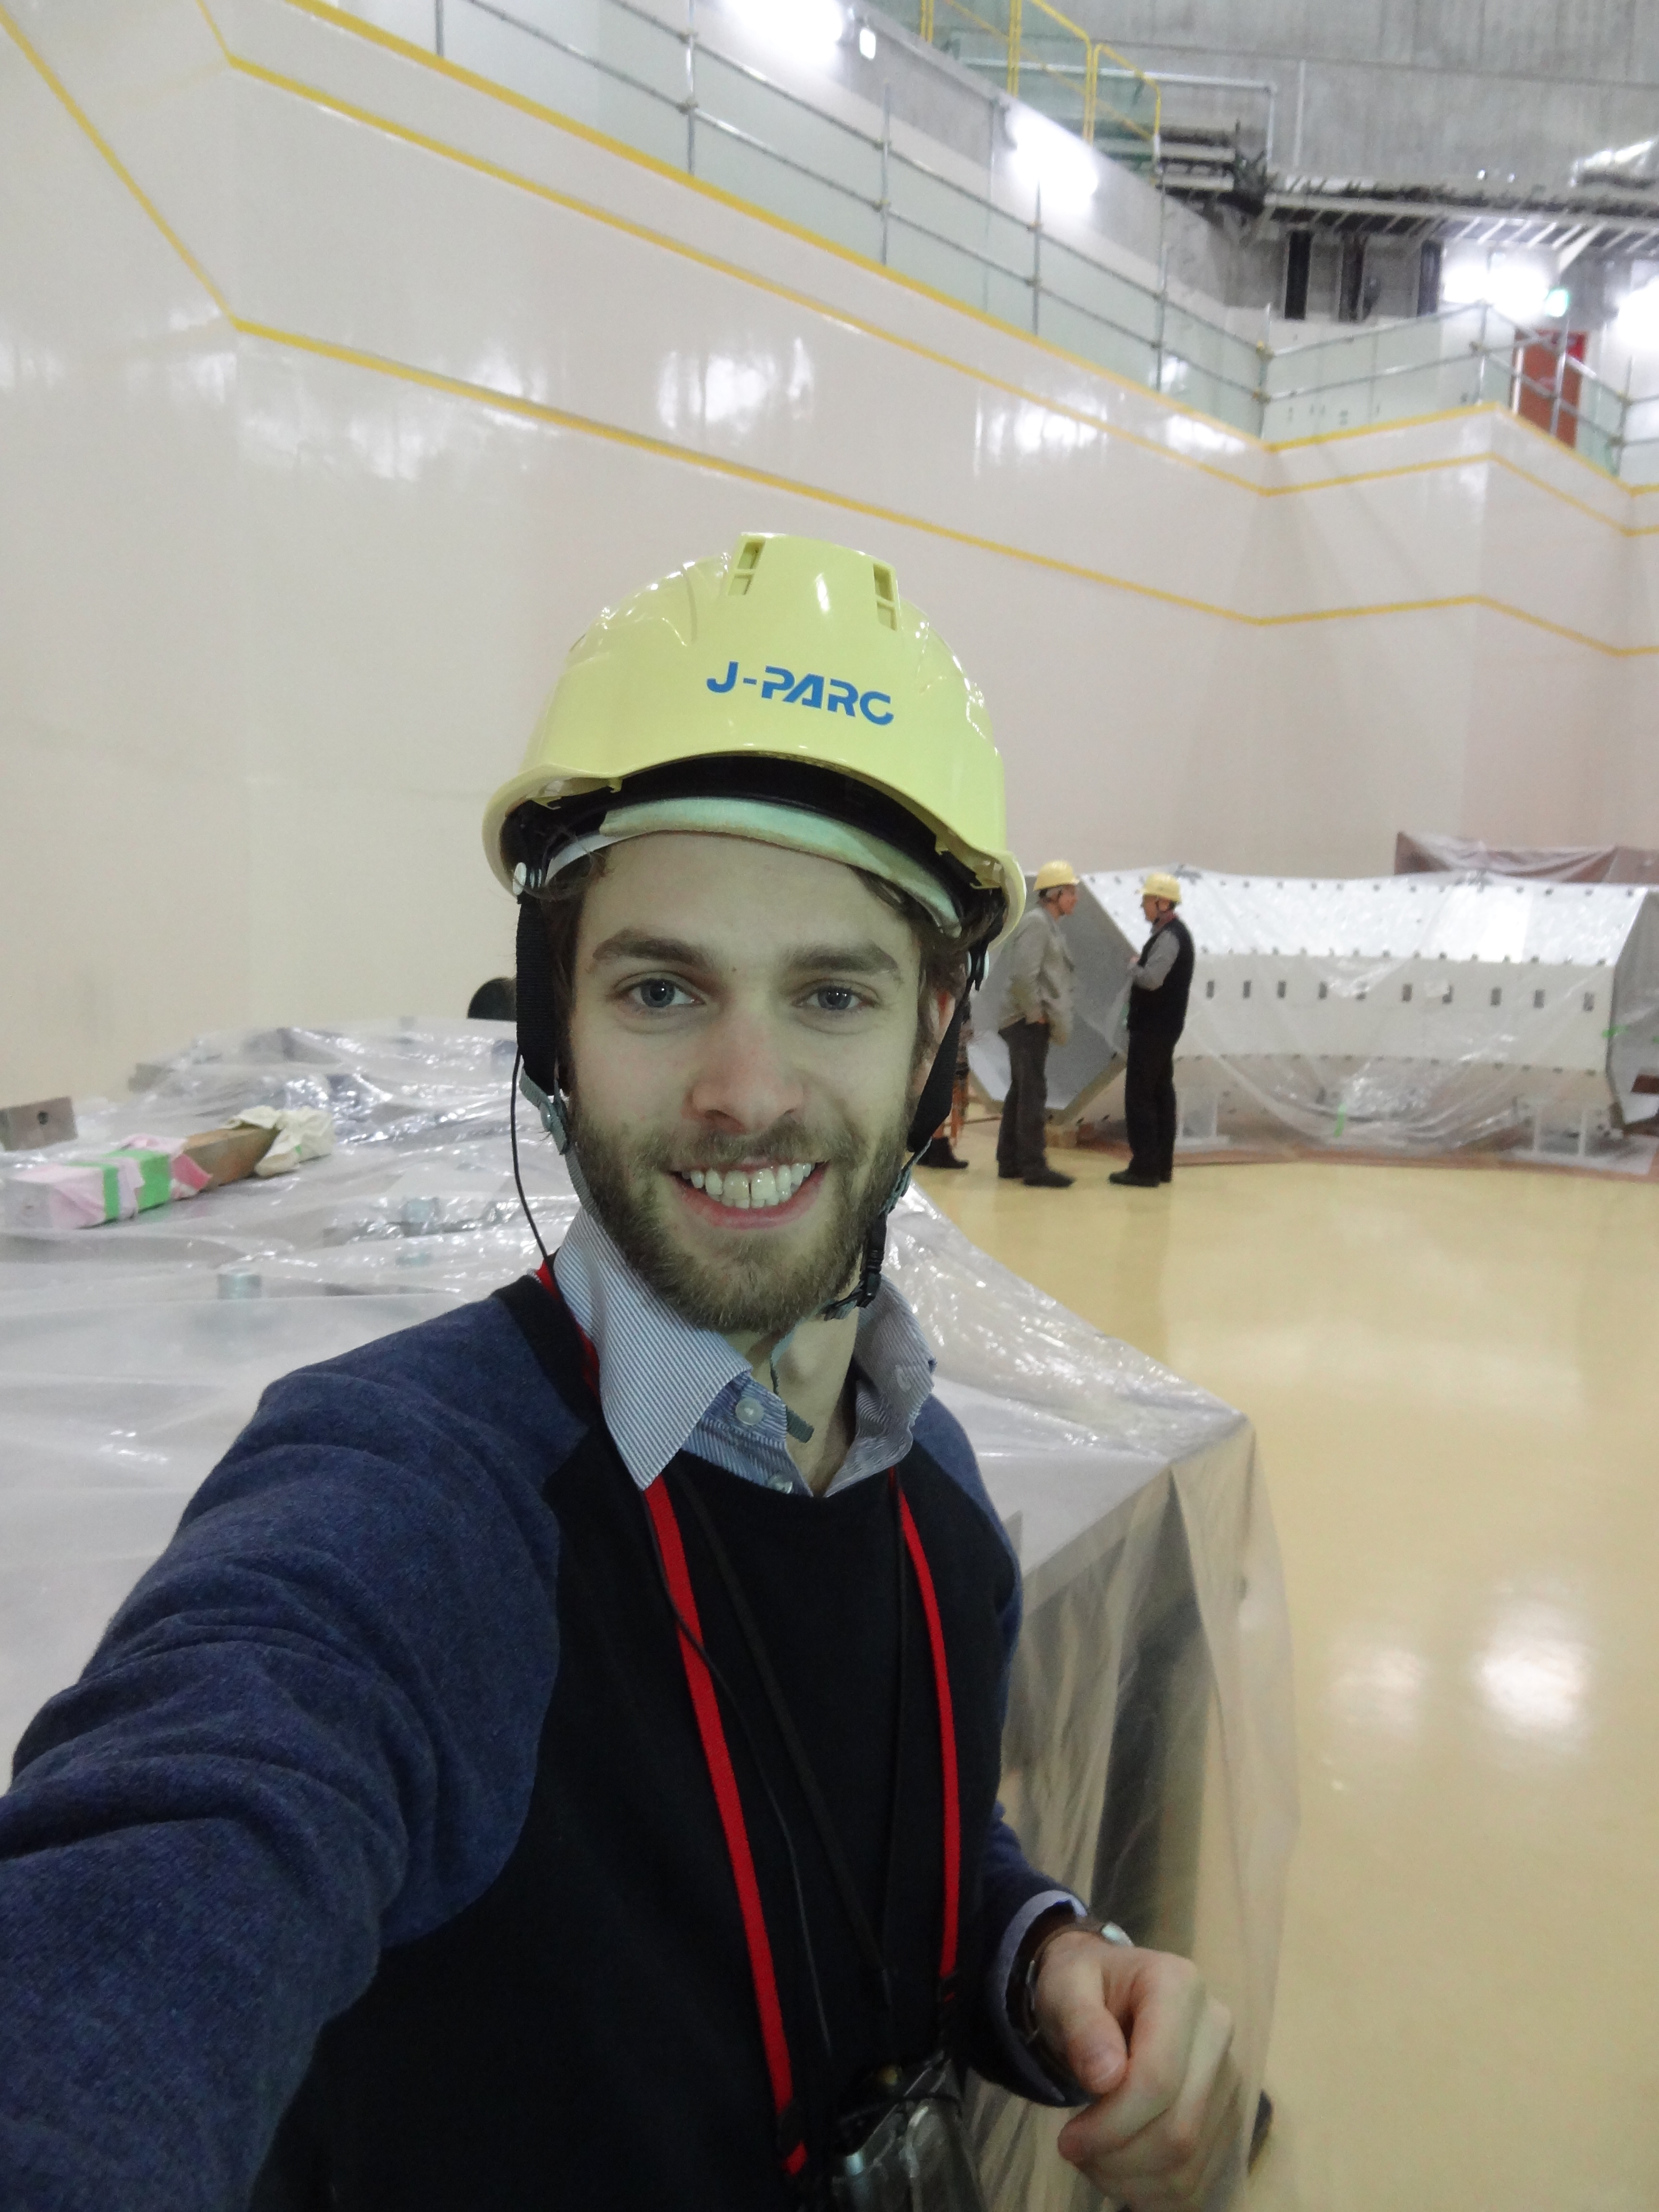
\includegraphics[width=0.29\textwidth]{figs/detector/status_photos/Hall_meVisit}}
\caption{\figlabel{detector:setup:facility}
Photographs of the experiment hall being constructed and first sections of beamline being installed.
}
\end{figure}
}

\newcommand{\FigStatusCyDet}{
\begin{figure}[p]
\centering
	\subfloat[][\figlabel{detector:setup:CyDet:stringing}]{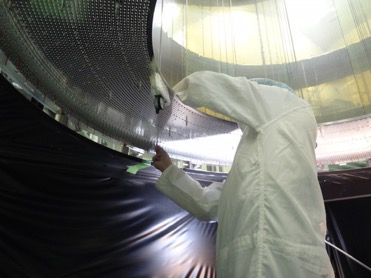
\includegraphics[width=0.52\textwidth]{figs/detector/status_photos/CDC-stringing.jpg}}\hspace{0.3cm}
\subfloat[][\figlabel{detector:setup:CyDet:outerWall}]{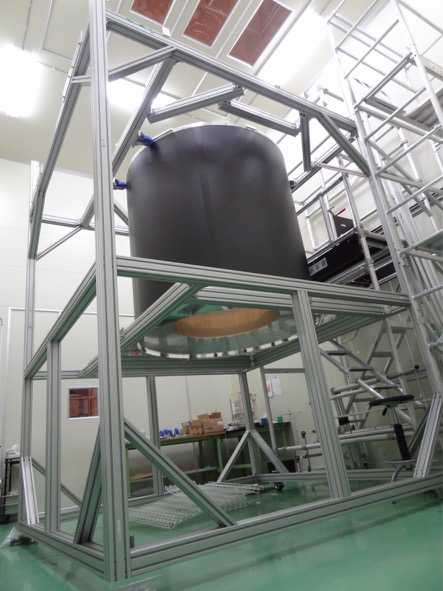
\includegraphics[width=0.29\textwidth]{figs/detector/status_photos/CDC-outerWall.jpg}}
\caption{\figlabel{detector:status:CyDet}
The CDC being assembled and strung.
}
\end{figure}
}

\newcommand{\FigStatusStrECAL}{
\begin{figure}[p]
\centering
\subfloat[][\figlabel{straw-production}Straw Tube Construction and Prototype Tracker]{%
       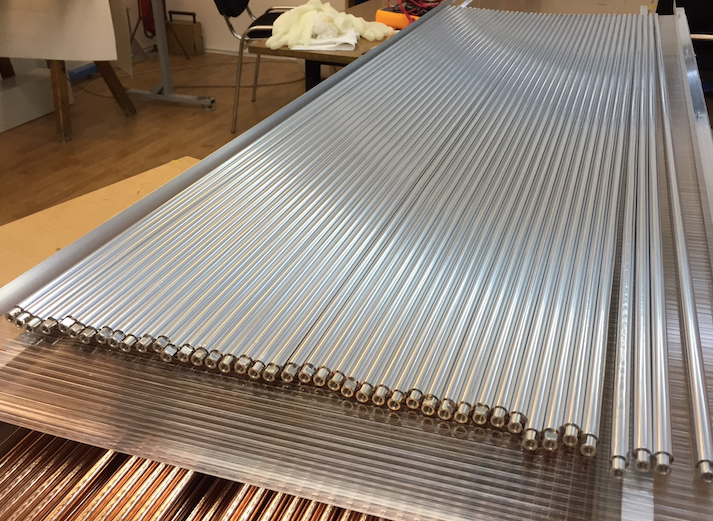
\includegraphics[height=0.2\textheight]{figs/detector/status_photos/StrawTrackerProduction.jpg}\hspace{4pt}%
       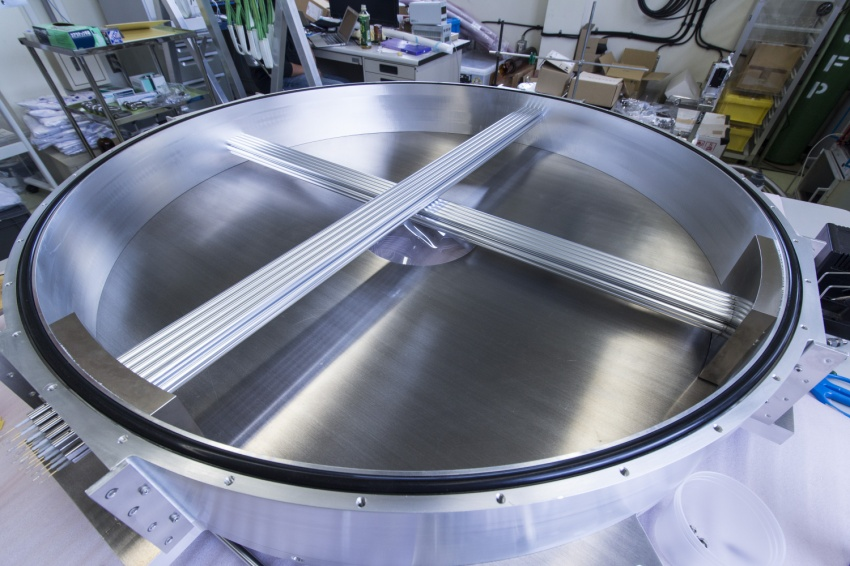
\includegraphics[height=0.2\textheight]{figs/detector/status_photos/StrawTrackerPrototype.jpg}
}\\
\subfloat[][\figlabel{ecal-production}Crystal Wrapping and Test Beam]{%
       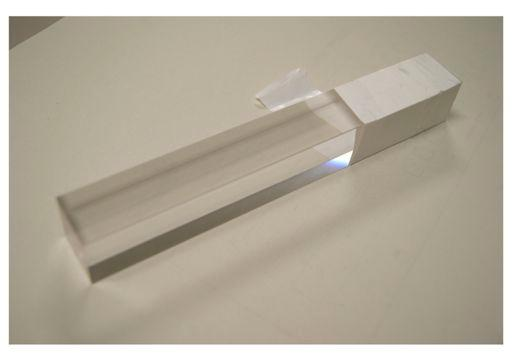
\includegraphics[height=0.19\textheight,trim=5ex 4ex 5ex 4ex,clip]{figs/detector/status_photos/ECAL-crystal}\hspace{4pt}%
       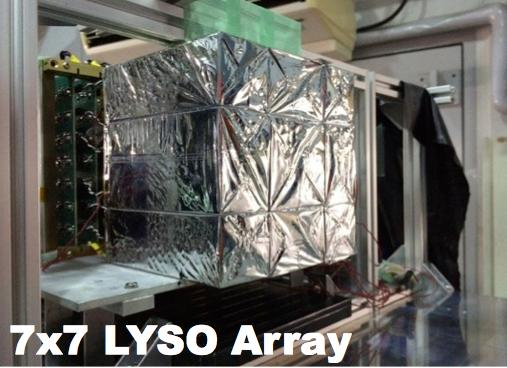
\includegraphics[height=0.19\textheight,trim=0 2cm 0 0,clip]{figs/detector/status_photos/ECAL-testBeam}
}
\caption{\figlabel{detector:status:StrECAL}
Research and development for the \ac{StrECAL} showing both the individual straws or crystal and a prototype set-up used at test beams to characterise the sub-detectors.
}
\end{figure}
}
